% !TeX root = ../../main.tex
\chapter{Contribution}
\label{chapter:contribution}

This chapter presents the conceptualization of a proposed Scala-based architecture for enabling the development of cross-platform, polyglot and distributed libraries and frameworks.

Its discussion is structured as follows.
%
First, the intents and application scenarios motivating the proposed architecture are discussed.
%
Subsequently, the corresponding requirements and constraints are formalized.
%
Thereafter, the elements composing the architecture are presented.
%
Finally, the implications of adopting this design are analyzed.

\section{Intents}

The intents of the proposed architecture are to enable the development of distributed Scala libraries and frameworks to be both \textit{cross-platform}, that is, able to run on multiple platforms and runtimes; and \textit{polyglot}, that is, designed to be able to interoperate with its public interface from multiple programming languages.
%
Both intents are achieved while maintaining a unified version of the components implementing the application logic of the software product.

\section{Application scenarios}

This architecture is well suited when the following scenarios arise:
%
\begin{itemize}
    \item \textbf{Application environment heterogeneity.} The library or framework implements functionalities that should be deployed and executed in heterogeneous environments, spanning across multiple platforms and runtimes. This may arise from the heterogeneity of end-user deployment environments or the requirement that platform and runtime selection remain contingent upon the specific application context in which the library is used.
    \item \textbf{Polyglot end-user base.} The library is designed for developers working across different programming languages, enabling team diversity, facilitating integration with existing codebases in various languages, and leveraging language-specific features and ecosystems.
    \item \textbf{Unified application logic.} The library exposes its functionalities through a unified API, regardless of the target platform, runtime or programming language. This ensures behavioral consistency across all supported environments, enabling seamless interoperability between programs utilizing the library.
\end{itemize}

\section{Requirements}

Requirements formally describe the boundary of applicability of the proposed architecture.
%
These can be categorized into \textit{user}, \textit{system} and \textit{implementation} requirements and address two types of stakeholders: \textit{library users}, who are developers intending to use the libraries and frameworks designed following the proposed architecture; and \textit{library developers}, who design and implement such libraries and frameworks.

\subsubsection{User requirements}

\begin{enumerate}[label=U\arabic*.]
    \item Library users must be able to interact with the library from multiple programming languages through a consistent API, benefiting from language-specific ecosystem features. Supported languages include:
    %
    \begin{itemize}
        \item Scala;
% todo: \item Java;
        \item JavaScript; 
        \item TypeScript;
        \item C and C++.
    \end{itemize}
    %
    \item The library must support execution across heterogeneous platforms and runtimes to accommodate diverse library user deployment environments. Library users must be able to implement their own solution by building upon the library's core functionalities:
    %
    \begin{itemize}
        \item using Scala, with deployments possibly spanning across the following platforms and runtimes:
        %
        \begin{itemize}
            \item JVM;
            \item JavaScript environments, both browser-based and server-side (Node.js);
            \item Native environments, including desktop, server, and System on Chip (SoC) devices running on 64-bit and ARM architectures.
        \end{itemize}
        %
        \item using other supported languages, targeting their respective platforms. Except for Scala, Library Users should not need to compile code written for one platform to run on another; e.g., compiling C code to run on Node.js.
    \end{itemize}
    \item Library users can distribute the execution of their application-specific code across multiple machines, with each node potentially running on different platforms, runtimes, and programming languages. The library provides distributed communication mechanisms that enable seamless interoperability and coordination among them.
\end{enumerate}

\subsubsection{System requirements}

\begin{enumerate}[label=S\arabic*.]
    \item Library developers must be able to implement the library logic once and reuse it across all supported platforms and runtimes. Modifications to the library logic are automatically reflected across all target platforms and runtimes.
    \item Library API must be consistent across all supported languages and behaves uniformly regardless of the target platform, runtime and programming language.
\end{enumerate}

\subsubsection{Implementation requirements}

\begin{enumerate}[label=I\arabic*.]
    \item Developers implement the library taking advantage of the full Scala language features and capabilities, enabling them to harness functional programming, type-safe abstractions, expressive syntax and compositional design patterns to facilitate the development of robust, scalable and distributed software systems.
    \item The bridge layer between programming languages should not rely on remote procedure calls (RPC) or inter-process communication (IPC) mechanisms to not incur in the performance penalties associated with these techniques.
\end{enumerate}

\section{Constraints}

The proposed architecture imposes a fundamental constraint that significantly influences architectural decisions: all dependencies must support cross-compilation to all target platforms.
%
Where such multi-platform support is unavailable, platform-specific implementations must be provided explicitly to bridge the abstraction gap.
%
If an existing Scala library heavily relies on platform-specific dependency or its design is tightly coupled with a specific platform or runtime, adapting it to the proposed architecture may prove impractical or require substantial reengineering efforts.
%
For example, a distributed Scala library built on Akka\footnote{\url{https://akka.io}} and utilizing its remoting and clustering capabilities would require substantial redesign to support multi-platform execution, as Akka targets only the JVM. 
%
However, this challenge can be mitigated if these dependencies have been carefully abstracted as replaceable components.
%
Furthermore, when platform-specific dependencies provide critical non-functional properties---such as fault tolerance or scalability---that multi-platform alternatives cannot yet match, adapting to a cross-platform architecture becomes not merely impractical but potentially unfeasible.
%
In these cases, the tight coupling to a specific platform represents an architectural constraint rather than an implementation detail, and the proposed architecture may not constitute a suitable approach for such libraries without revisiting their core design principles.

\section{Architectural elements}

The proposed architecture, presented in \Cref{fig:reference-architecture}, is composed of three main components:

\begin{enumerate}
    \item a \textbf{pure core module}, implementing the application logic of the library. This module is designed to be platform-agnostic and independent of any specific technology or runtime;
    \item a \textbf{cross-platform infrastructure module}, responsible for enabling the distribution of the library functionalities across multiple end nodes. This includes a \textbf{general cross-platform and polyglot serialization binding}, providing the capability to marshal and unmarshal data structures exchanged between different platforms, runtimes and programming languages;
    \item a \textbf{polyglot abstraction layer}, exposing a simplified and consistent interface API to library users through different programming languages.
\end{enumerate}

The core module and the cross-platform infrastructure module together constitute the \textit{Software Product}, which implements the library's core functionalities and delivers its primary value.
%
The polyglot abstraction layer, by contrast, forms part of the \textit{User Interface}, providing the programmatic interface through which library users interact with the software product using any of the supported programming languages.
%
This separation enables library users to interact seamlessly with the library in their preferred programming language, accessing its functionalities through native packages generated by the polyglot library abstraction layer.
%
Library developers, meanwhile, can focus on implementing the core logic without being concerned about language-specific details.

\begin{figure}
    \centering
    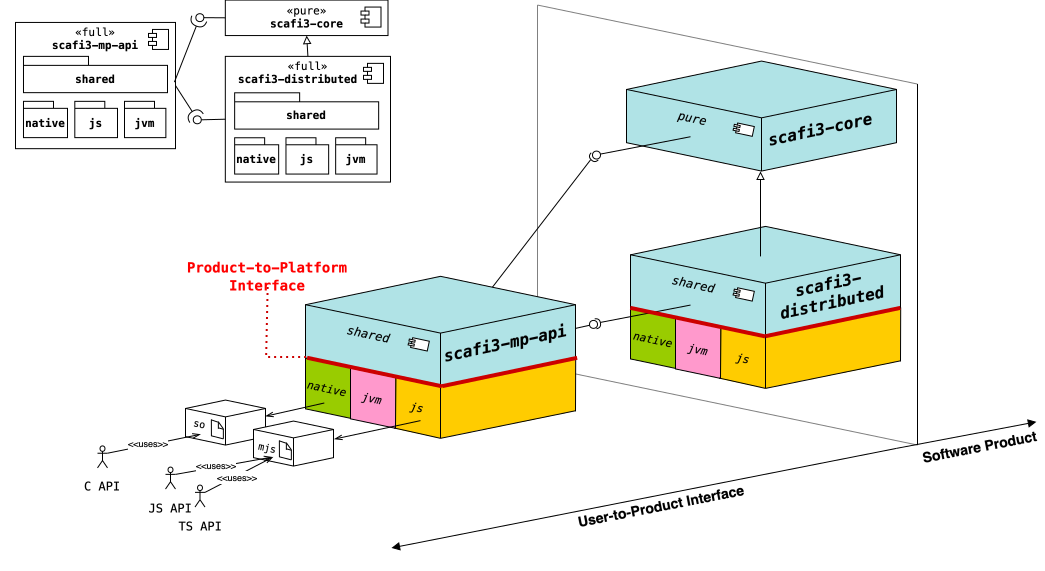
\includegraphics[width=\textwidth]{resources/img/architecture.pdf}
    \caption{Proposed reference architecture for cross-platform, polyglot and distributed Scala libraries and frameworks.}
    \label{fig:reference-architecture}
\end{figure}

Once applied, library users can take advantage of the library as depicted in \Cref{fig:architectural-workflow}.
%
They can implement their application logic directly in Scala, leveraging its full language features and capabilities and cross-compiling it to all target platforms and runtimes, by consuming the respective library artifact from a Central repository (e.g., Maven Central).
%
Alternatively, they can program their application logic in any of the supported programming languages, utilizing the corresponding artifacts generated by the polyglot abstraction layer and published to the respective platform-specific package repositories.

\begin{figure}
    \centering
    \includegraphics[width=\textwidth]{resources/img/architecture-workflow.pdf}
    \caption{Library usage workflow enabled by the proposed architecture.}
    \label{fig:architectural-workflow}
\end{figure}

\subsection*{Pure library core module}

The core module is the heart of the library, implementing its core application logic and functionalities in terms of domain modeling, business rules and application use cases.
%
Its architecture is deliberately designed to be both platform- and technology-agnostic, ensuring the core logic to be reusable across multiple execution environments without requiring any modification or adaptation.
%
This design can be achieved by adhering to the Hexagonal (Ports \& Adapters) Architectural pattern \cite{hexagonal}, which promote the decoupling of the core logic from external dependencies by defining clear interfaces (ports) and isolating the core logic from infrastructural concerns (adapters).

Implemented as a Scala pure multi-platform module, it enables the cross-compilation of the core logic to all target platforms and supported runtimes.

\subsection*{Cross-platform infrastructure module}

This is the component dealing with infrastructural concerns.
%
Despite the fact it is conceptually represented as a single module, depending on the complexity of the library and its requirements, it can be decomposed into multiple modules, each addressing specific infrastructural aspects.
%
Its core responsibilities include the implementation of a distributed communication mechanism and a general serialization binding.

\subsubsection*{Cross-platform distribution module}

For distributed communication, the library can leverage different underlying technologies and protocols depending on specific use cases and requirements, such as peer-to-peer or publish-subscribe messaging patterns. 
%
Regardless of the chosen communication model, the design must maximize code reuse across all supported platforms and runtimes.
%
This is achieved through well-defined \textit{Platform Interfaces} that abstract platform-specific capabilities and services, isolating them from the shared library logic. 
%
These interfaces are designed to satisfy both the library's functional requirements and the native paradigms of each target platform.
%
For example, the interfaces use asynchronous API patterns that can be uniformly implemented across all supported environments.
%
Platform-specific adapters then implement these interfaces, encapsulating only the minimal necessary platform-dependent code.
%
Whenever possible, existing multi-platform libraries and frameworks should be leveraged.
%
Conversely, when no suitable multi-platform library exists, custom platform-specific implementations must be developed by interacting directly with the underlying platform capabilities and ecosystem via Scala Native or Scala.js interoperability features.
%
In both cases, all implementation adapters must conform to the defined Platform Interfaces to ensure maintainability and facilitate the integration of alternative platform-specific implementations.

\subsubsection*{Polyglot serialization binding}

Concerning the serialization binding, it must be designed to be format-agnostic and interoperable across different programming languages and platforms. 
%
Format agnosticism is desirable to ensure flexibility and interchangeability of serialization formats, while cross-platform interoperability is a strict requirement.
%
Indeed, if the serialization format is not compatible across all supported languages and platforms, the library would not be able to consistently exchange messages between different end nodes, thus undermining its distributed nature.

Selecting a serialization format requires evaluating multiple factors.
%
Performance and efficiency trade-offs between textual and binary formats must be weighed against compatibility with all supported programming languages and platforms.
%
Additionally, the choice between schema-based and schema-less formats affects the flexibility and evolvability of serialized data structures.
%
A critical consideration is the degree of automation in serializer and deserializer generation: while automatic code generation simplifies development, it may limit the ability to define custom data types and structures that leverage language-specific abstractions.
%
This tension is particularly relevant given that different programming languages offer distinct abstractions that cannot always be straightforwardly mapped.

\vspace{-0.5em}
\subsection*{Polyglot library abstraction layer}

The polyglot abstraction layer exposes a uniform interface enabling cross-language interaction with the library's core functionalities. 
%
Two critical challenges converge to demand the presence of this layer: type system mismatches and limited type construct mapping.

\vspace{0.5em}
\noindent
\textbf{Type system mismatches.}
%
Mismatches arise because both Scala Native and Scala.js address language semantics differences by reifying them into new types.
%
For example, Scala.js introduce the \texttt{js.Map} type to represent JavaScript maps, distinct from Scala's \texttt{Map} type.
%
Similarly, both projects define platform-specific types for interoperability: Scala.js provides \texttt{js.UndefOr} for nullable types and \texttt{js.FunctionN} for JavaScript functions, while Scala Native uses \texttt{null} for nullable types and \texttt{CFuncPtrN} for C function pointers.
%
While this approach preserves type-safety, guarantees correct usage, and makes users aware of the underlying platform constraints and peculiarities, it prevents exposing a unified API across all supported languages.
%
Without this layer, library developers would be forced to create different facades for both JavaScript and C, leading to code duplication, increased maintenance effort and potential inconsistencies.

\vspace{0.5em}
\noindent
\textbf{Limited type construct mapping.}
%
This is a consequence of the fact that only a subset of Scala type constructs can be mapped and exposed to JavaScript and C.
%
Indeed, while Scala code can be cross-compiled to both JavaScript and native binaries, not all Scala type constructs have a direct counterpart in these target languages.
%
Consequently, the ability to cross-compile a Scala construct does not guarantee it can be exposed to or utilized by other programming languages.
%
For example, Scala's rich type system includes Path Dependent Types \cite{path-dependent-types} and Implicit parameters \cite{scala-contextual-abstractions}, which have no direct equivalents in other programming languages.

The proposed polyglot abstraction layer tackles these challenges by introducing \textit{abstract, language-independent types} that are \textit{isomorphic} to Scala types. 
%
They are decoupled from any specific programming language or platform, yet maintain a one-to-one mapping to corresponding Scala types.
%
Referred to as \textbf{Portable Types}, these are then instantiated within each supported platform, providing language-specific implementations and dedicated bidirectional conversion between them and their corresponding Scala equivalents.

Using this approach the core library API is exposed to library users through portable types, providing simplified interfaces as a thin wrapper around the core library API.
%
Within the polyglot abstraction layer, the conversion between portable types and the corresponding Scala types used by the core library is handled.
%
The exposed interfaces---referred to as \textbf{Portable Libraries}---can then be exported, packed and distributed as native packages for each supported programming language, since, during cross-compilation, Portable Types are translated to the corresponding language-specific types.
%
Essentially, Portable Types act as a small standard library for this module, written in a "de-powered" version of Scala that is limited, in its expressiveness, to the constructs that can be mapped and exported to all supported programming languages.

Beyond collection-types, each Portable Library can extend the set of portable types by defining domain-specific data types to model the library domain, mirroring standard type definition practices.
%
These must maintain the same isomorphic mapping principle, ensuring seamless conversion between platform-specific incarnations and Scala types.

Implementation-wise, Portable Libraries are structured as a thin wrapper around the core library API, using only Portable Types in their public interface.
%
Internally, the logic is delegated to the core library after converting Portable Types to their corresponding Scala types using the provided isomorphic mappings, as shown in \Cref{fig:portable-types-mapping}.
%
\begin{figure}[htbp]
    \centering
    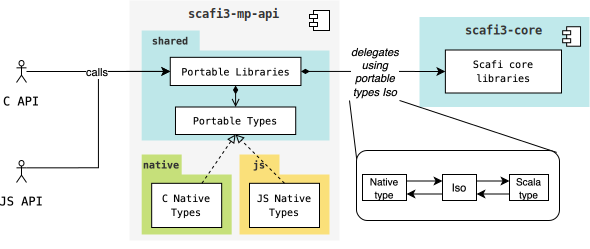
\includegraphics[width=\textwidth]{resources/img/portable-types-mapping.pdf}
    \caption[Language-Agnostic API access through Portable Libraries and isomorphic type mappings]{Clients interact with the core library API through Portable Libraries, which expose a simplified interface towards the core library using Portable Types. Thanks to language-specific instantiations of Portable Types and appropriate isomorphic mappings, Portable Libraries simply delegate to the core library API their implementation.}
    \label{fig:portable-types-mapping}
\end{figure}

Notably, the polyglot abstraction layer must account for fundamental differences among all supported programming languages, modeling and abstracting these distinctions to present them through a unified API.
%
These differences encompass:
%
\begin{itemize}
\item error handling mechanisms, such as exceptions in JavaScript and error codes in C;
\item API design paradigms, including asynchronous and synchronous styles;
\item equality and hashing semantics;
\item memory management models.
\end{itemize}
%
\Cref{chapter:scafi3-arch-reification} presents how Portable Types and Portable Libraries can be implemented to model and abstract these language-level differences.

\section{Consequences}

This architecture enables the development of cross-platform, polyglot and distributed Scala libraries and frameworks by addressing the challenges associated with platform heterogeneity, language interoperability and distributed communication.
%
Its main focus is to maximize code sharing and reuse across all supported platforms and languages, and provide a consistent and unified API to library users.

Some considerations and trade-offs are presented hereafter.
%
\begin{enumerate}
    \item \textbf{API Maintenance.} While every code change in the core library is automatically reflected across all supported platforms and runtimes, the addition of new API functionalities requires extending the polyglot abstraction layer to expose the new features to library users. Despite not being a significant overhead, since the polyglot abstraction layer is designed to be thin and minimal, it still requires some additional effort to maintain and evolve.
    \item \textbf{Performance Overhead.} Interoperability across programming languages is achieved through type conversion, which may introduces performance overhead if compared with native implementations, particularly when handling complex data structures or large data volumes. However, this overhead is significantly lower than RPC or IPC approaches, which require additional serialization and boundary crossing costs.
    \item \textbf{Data Expressiveness.} The expressiveness of exchanged messages between nodes is limited to the capabilities of the adopted cross-platform and polyglot serialization format. This normally does not pose significant limitations since exchanged messages are represented as \textit{records}—--immutable data classes composed of fields with no additional behavior. However, complex data structures or language-specific constructs may not be fully representable and may require simplifications or alternative representations.
\end{enumerate}
